\documentclass[a4paper,12pt]{report}

\usepackage{fullpage}
\usepackage{microtype}
\usepackage{graphicx}
\usepackage[utf8]{inputenc}
\usepackage[frenchb]{babel}
\usepackage{hyperref}
\usepackage{wrapfig}
\usepackage{mathtools}
%\usepackage{draftwatermark}
%\SetWatermarkScale{6}

\usepackage[section]{placeins}
\usepackage{float} 

%neural networks
\usepackage{tikz}
\def\layersep{2.5cm}

\renewcommand{\baselinestretch}{1.3}
%\renewcommand{\contentsname}{Sommaire}
\newcommand{\HRule}{\rule{\linewidth}{0.5mm}}


\author{Kevin Furet-Stricher}
\title{Atelier Indexation d'Images}



\begin{document}


%\maketitle
\begin{titlepage}
	\begin{center}

	~\\[1.5cm]

	
\includegraphics[width=0.4\textwidth]{./logo}~\\[1cm]
	\textsc{\Large Université de Cergy-Pontoise}\\[1.5cm]

	\textsc{\large Atelier}\\[0.5cm]

	% Title
	\HRule \\[0.4cm]
	{ \LARGE \bfseries Indexation d'Images \\[0.4cm] }

	\HRule \\[1.5cm]

	% Author and supervisor
	\begin{minipage}{0.4\textwidth}
	\begin{flushleft} 
	\emph{Rédigé par :}\\
	Lise \textsc{Aubin}\\
	Kevin \textsc{Furet Stricher}
	\end{flushleft}
	\end{minipage}
	\begin{minipage}{0.4\textwidth}
	\begin{flushright} 
	\emph{Encadré par :} \\
	Dan \textsc{Vodislav}\\
	Ghilès \textsc{Mostafaoui}\\
	\end{flushright}
	\end{minipage}
	
	\vfill
	
	% Bottom of the page
	{\large septembre 2016}
	
	\end{center}
\end{titlepage}

\tableofcontents

\chapter{Introduction}
	\section{Sujet}
	\section{Organisation}

\chapter{Présentation globale}

	\section{Architecture}
	\subsection{Schéma global}
	\subsection{Traitement d'images : Executable C}
	\subsection{Interface d'échange : Fichiers descripteurs}
	\subsection{Base de données Oracle}
	\subsection{IHM : Programme Java}
	
	\section{Fonctionnalités}
	
\chapter{Analyse détaillée}

	\section{Traitement d'images et indexation}
	
	\section{Base de données et requêtes d'exploitation}

Les critères de ressemblance que nous avons choisis pour trouver les images similaires ont été les suivants:
\begin{enumerate}
\item La couleur
\item Le nombre de pixels de contour
\item L'histogramme des niveaux de gris
\end{enumerate} 

Pour la couleur, nous nous servons des taux de rouge, de bleu et de vert des images stockées dans la base. Afin de trouver les images similaires à une image de référence, nous cherchons les images ayant des taux les plus proches de celle-ci.

Pour la forme, nous utilisons le nombre de pixels de contour. De même que pour la couleur, nous cherchons les images ayant un nombre de pixels de contour proche de l'image de référence.

Pour l'histogramme, nous cherchons les images ayant une distance de bhattacharya (voir formule ci-dessou)  entre leur histogramme et celui de l'image de référence la plus petite possible.

\paragraph{}Bhattacharya distance :
\begin{center} 
$d = \sum\limits_{i=0}^n\sqrt{\frac{p(x)q(x)}{\sum\limits_{i=0}^n p(x)\sum\limits_{i=0}^n q(x)} }$ 
\end{center} 

Pour les requêtes avec Oracle nous avons utilisé les signatures et la méthode isSimilar() qui peut être paramétrisée pour trouver les images ayant la même couleur, la même forme etc.

Les résultats que nous avons obtenu se trouve ci-dessous.

\begin{center}
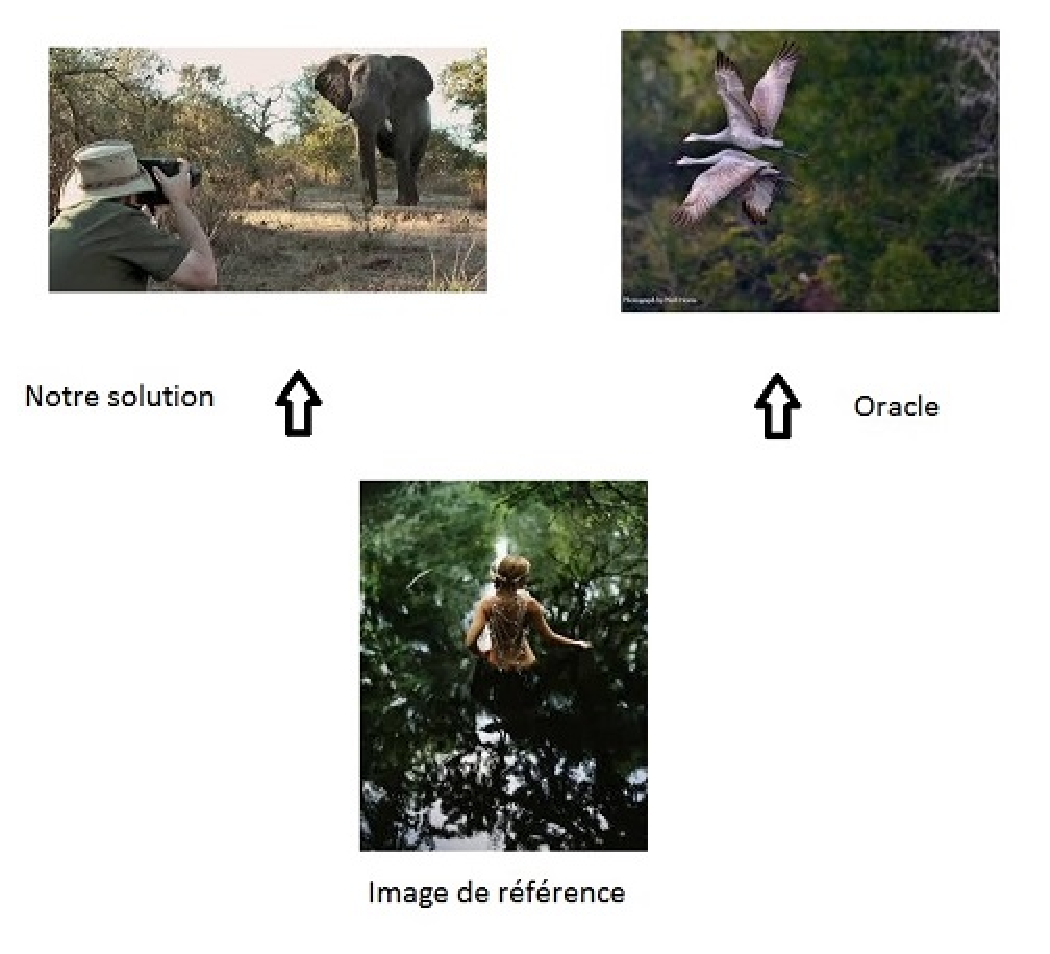
\includegraphics[scale=0.55]{resultatColor.eps}
\hspace{5pt}
\captionof{figure}{Résultat avec la couleur comme critère de ressemblance}
\end{center}

\begin{center}
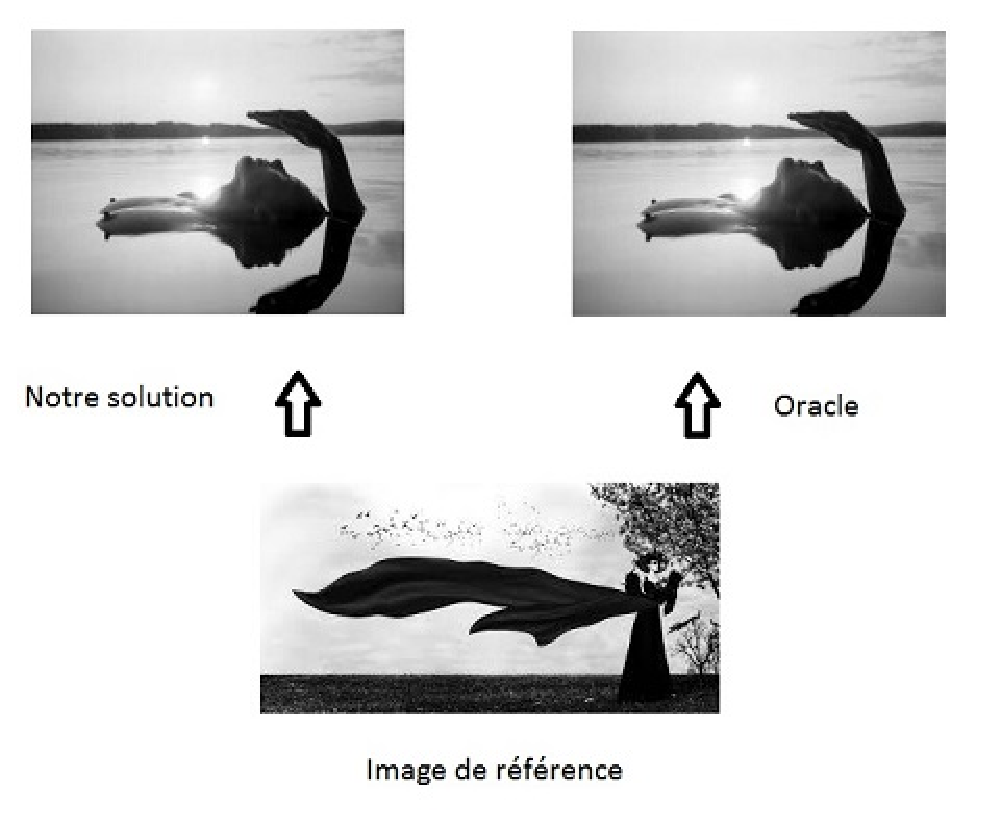
\includegraphics[scale=0.55]{resultatShape.eps}
\hspace{5pt}
\captionof{figure}{Résultat avec le nombre de pixels de contour comme critère de ressemblance}
\end{center}

\begin{center}
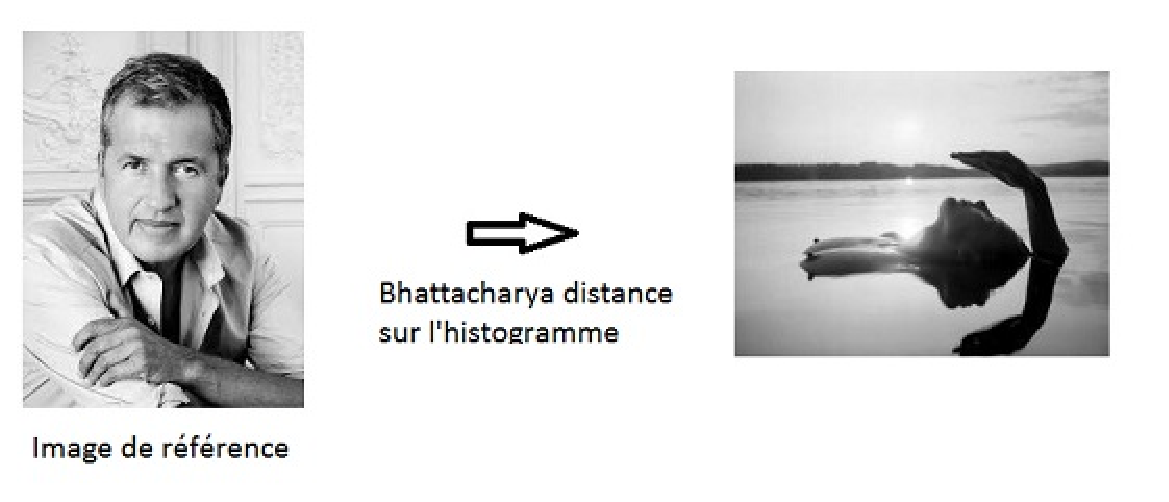
\includegraphics[scale=0.55]{resultatHist.eps}
\hspace{5pt}
\captionof{figure}{Résultat avec l'histogramme comme critère de ressemblance}
\end{center}

Avec le critère de couleur, la méthode d'Oracle obtient en moyenne des résultats plus précis. En effet, les teintes dans les images résultats sont plus proches que celle que nous trouvons avec notre méthode. Nous en déduisons que pour obtenir un résultat plus précis il faudrait utiliser d'autres critères que simplement les taux de couleur. De plus, notre méthode pour calculer les taux utilise des seuils nous permettant de décidé à quelle couleur appartient le pixel (rouge, bleu, vert, gris) ce qui ne permet de pas de souplesse et demande une paramétrisation du seuil fine.
Avec critère basé sur le nombre de pixels de contour, nous trouvons des résultats très proches de ceux donnés par Oracle.

Pour ce qui est du critère sur l'histogramme, nous n'avons pas de comparatif avec Oracle et il est difficile de déterminer visuelement la pertinence de nos résultats.


Nous avons comparé les temps d'execution entre les requêtes utilisant les méthodes Oracle et nos méthodes.

\begin{table}[ht]
\centering
\resizebox{\textwidth}{!}{
\begin{tabular}{|c|c|c|}
\hline
Requêtes & Temps d'execution oracle (s) & Temps d'execution de notre méthode (s) \\
\hline
Couleur & 0.15 & 0.04 \\
\hline
Nombre de pixels de contour & 0.12 & 0.05 \\
\hline
histogramme & - & 0.65 \\
\hline
\end{tabular}}
\caption{Tableau de comparaison des temps d'execution} 
\end{table} 

Il s'est avéré que nos méthodes ont été plus rapides ce qui peut s'expliquer par le faite que nos traitements sont moins complexes que ceux effectués par Oracle.

	
\chapter{Conclusion}

\end{document}